\section{Results}
\label{sec:result}
% STDP-like paper
The model was evaluated on the MNIST dataset.
According to the authors of \cite{STDP_like}, the dataset is a suitable Benchmark for the \ac{SNN} model, 
since it provides different difficulty levels of categorization.
The authors of \cite{STDP_like} emphasise that the MNIST dataset less complex than biological vision.

The addition to accuracy with regard to the classification of the MNIST dataset impulses \cite{STDP_like} presents \ac{RT} distributions.
\ac{RT} is defined as the time between the presentation of a stimulus and the response (i.e. the first pool to reach the descision pool).
Usually, the \ac{RT} of misclassified digits is higher than the \ac{RT} of correctly classified digits.
However, the network also makes fast errors.
The results were verified with the Kolmogorov-Smirnov test, 
indicating that the correctly and misclassified \ac{RT} distributions are significantly different, 
whereas as the distributions for stimuli from the training and test set were not.
The Kolmogorov-Smirnov test \cite{Kolmogorov_Smirnov} is a non-parametric test for evaluating whether two samples came from the same distribution function.

The authors of \cite{STDP_like} compare the performance of the \ac{SNN} model for different training set sizes $n_{train}$.
They find that the network is able to generalize well if the training set size is sufficiently large.
The optimum training set size $n_{train} = 1000$ produced not remarkably higher misclassifaction rates than bigger training set sizes.
The most frequent misclassification was the digit nine as a zero.


% Original STDP paper
In \autoref{img:test_acc} the authors compare the performance of the \ac{SNN} model consisting of different numbers of excitatory neurons and different learning rules.
The standard deviation of the test accuracy is indicated by the error bars.
The black line denotes power-law weight dependence \ac{STDP}, the red one denotes exponential weight dependence \ac{STDP}, 
the green one indicates pre-and-post \ac{STDP}, wheras the blue line's learning rule is triplet \ac{STDP}.
The differences between these learning rules are explained in \cite{SNN}.
The visualization suggests that highest number of excitatory neurons (i.e. 6400) produces the best results for all learning rules.
The authors also study propose possible reasons for the distribution of misclassified digits proposed in \autoref{img:error_analysis}.
The most common misclassification was the digit four as a nine.

\begin{figure}[http]
    \begin{minipage}[b]{.5\linewidth}
         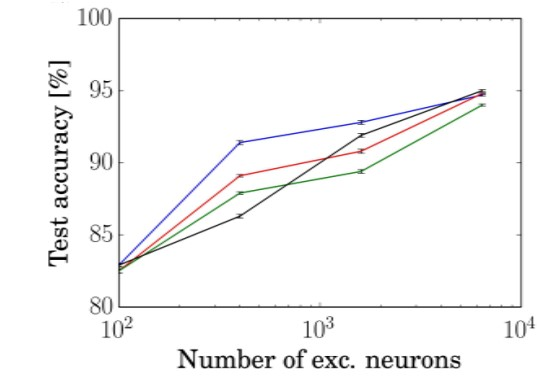
\includegraphics[width=\linewidth]{pictures/num_exc_neurons_test_acc.jpg}
         \caption{Test accuracy for different learning rules (colored lines) and different number of excitatory neurons from \cite{SNN}.}
         \label{img:test_acc}
    \end{minipage}
    \hspace{0.06\linewidth}% Abstand zwischen Bilder
    \begin{minipage}[b]{.4\linewidth}
         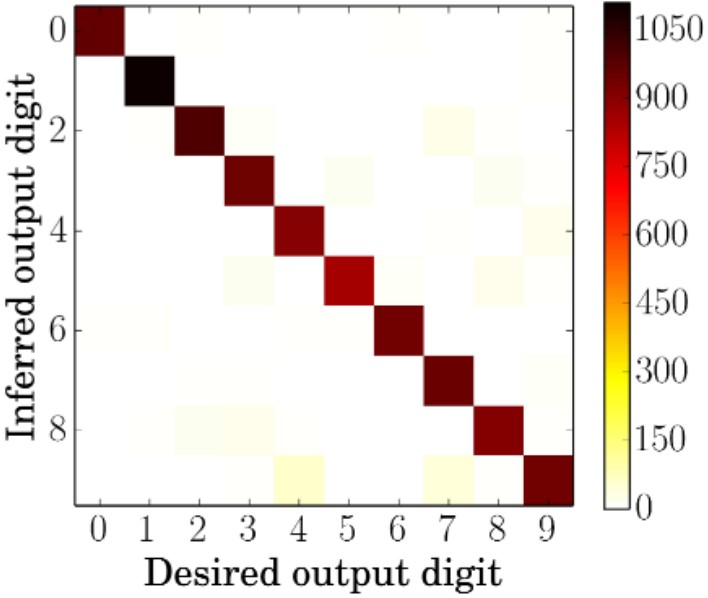
\includegraphics[width=\linewidth]{pictures/error_analysis_confusion_matrix.jpg}
         \caption{Confusion matrix presenting the average results over ten presentations of the 1000 MNIST test set digits from \cite{SNN}.}
         \label{img:error_analysis}
    \end{minipage}
\end{figure}

\begin{table}[]
    \begin{tabular}{|l|l|l|l|}
    \hline
    \textbf{Training type} & \textbf{(Un-) Supervised}    & \textbf{Learning rule}               & \textbf{Performance range} \\ \hline
    Rate-based             & Supervised                   & different                            & 90-99 \%                   \\ \hline
    Spike-based            & Supervised                   & different incl. calcium variable & 91-96 \%                   \\ \hline
    Spike-based            & Unsupervised                 & rectangular/ exponential \ac{STDP}        & 93-95 \%                   \\ \hline
    \end{tabular}
    \caption{Summary of methods compared in \cite{SNN}.}
    \label{tab:different-training-types}
\end{table}

The authors of \cite{SNN} include a table visualizing performances of different \acp{SNN}.
A summary of the types compared is given in \autoref{tab:different-training-types}.
Rate-based learning methods adchieve the best results.
Supervised methods imply the usage of a teaching signal.
The last learning rule from \autoref{tab:different-training-types} denotes the shape of the \ac{STDP} time window.
The calcium variable \cite{STDP_hebbian} is occasionally used to model the influence of the $Ca^{2+}$ level on activation neurons observed in biology:
A large $Ca^{2+}$ rise are associated with \ac{LTP}, whereas modest $Ca^{2+}$ rise may result in \ac{LTD}.

The authors of \cite{SNN} criticise, since neuron which are not in their refactory period can integrate incoming excitatory potentials and thus, 
increase their chance of firing possibly not all neurons have the same chance of firing after the refactory period.

Since the authors of \cite{SNN} have tested multiple different \ac{STDP} rules, as well as different training set sizes, 
they point out their model's robustness and good performance in a variaty of different situations, 
due to the competetion among the neurons resulting in dissimilar receptive fields.
Moreover, the authors of \cite{SNN} argue that their model is more biologically plausible.